\section{Temporal Constructs in the Vortex Æther Model (VAM)}\label{sec:temporal-constructs-in-the-vortex-ther-model-(vam)}

\begin{abstract}
This appendix defines and formalizes temporal constructs crucial to the Vortex Æther Model (VAM). By introducing a structured temporal ontology—from absolute universal time (Æther-Time) to locally measurable constructs (Chronos-Time, Swirl Clocks, Vortex Proper Time) and critical transition events (Kairos Moments)—we clarify the dynamics of temporality within structured vortex fields. These constructs form the temporal-topological triad supporting VAM's description of mass, gravity, and quantum phenomena.
\end{abstract}

\subsection{Hierarchical Temporal Ontology}

VAM utilizes a layered temporal ontology illustrated in Figure~\ref{fig:temporal_swirl}:
\begin{center}
\begin{tcolorbox}[
  colback=gray!10,
  colframe=black,
  width=0.9\textwidth,
  sharp corners=southwest,
  boxrule=0.5pt,
  before skip=10pt,
  after skip=10pt,
  title=\textbf{Table: Ætheric Time Modes in the Vortex Æther Model},
  fonttitle=\bfseries,
]
\renewcommand{\arraystretch}{1.25}
\begin{tabularx}{@{}lll@{}}
  \(\mathcal{N}\)     & \textbf{Aithēr-Time}         & Absolute causal background \\
  \(\nu_0\)           & \textbf{Now-Point}           & Localized universal present \\
  \(\tau\)            & \textbf{Chronos-Time}        & Measured time in the æther \\
  \(S(t)\)            & \textbf{Swirl Clock}         & Internal vortex phase memory \\
  \(T_v\)             & \textbf{Vortex Proper Time}  & Circulation-based duration \\
  \(\mathbb{K}\)      & \textbf{Kairos Moment}       & Topological transition point \\
\end{tabularx}
\end{tcolorbox}
\end{center}
\footnote{\(\Xi_0\) denotes the stationary reference frame of the universal superfluid æther. All temporal constructs evolve relative to this frame.}


\begin{figure}[H]
    \centering
    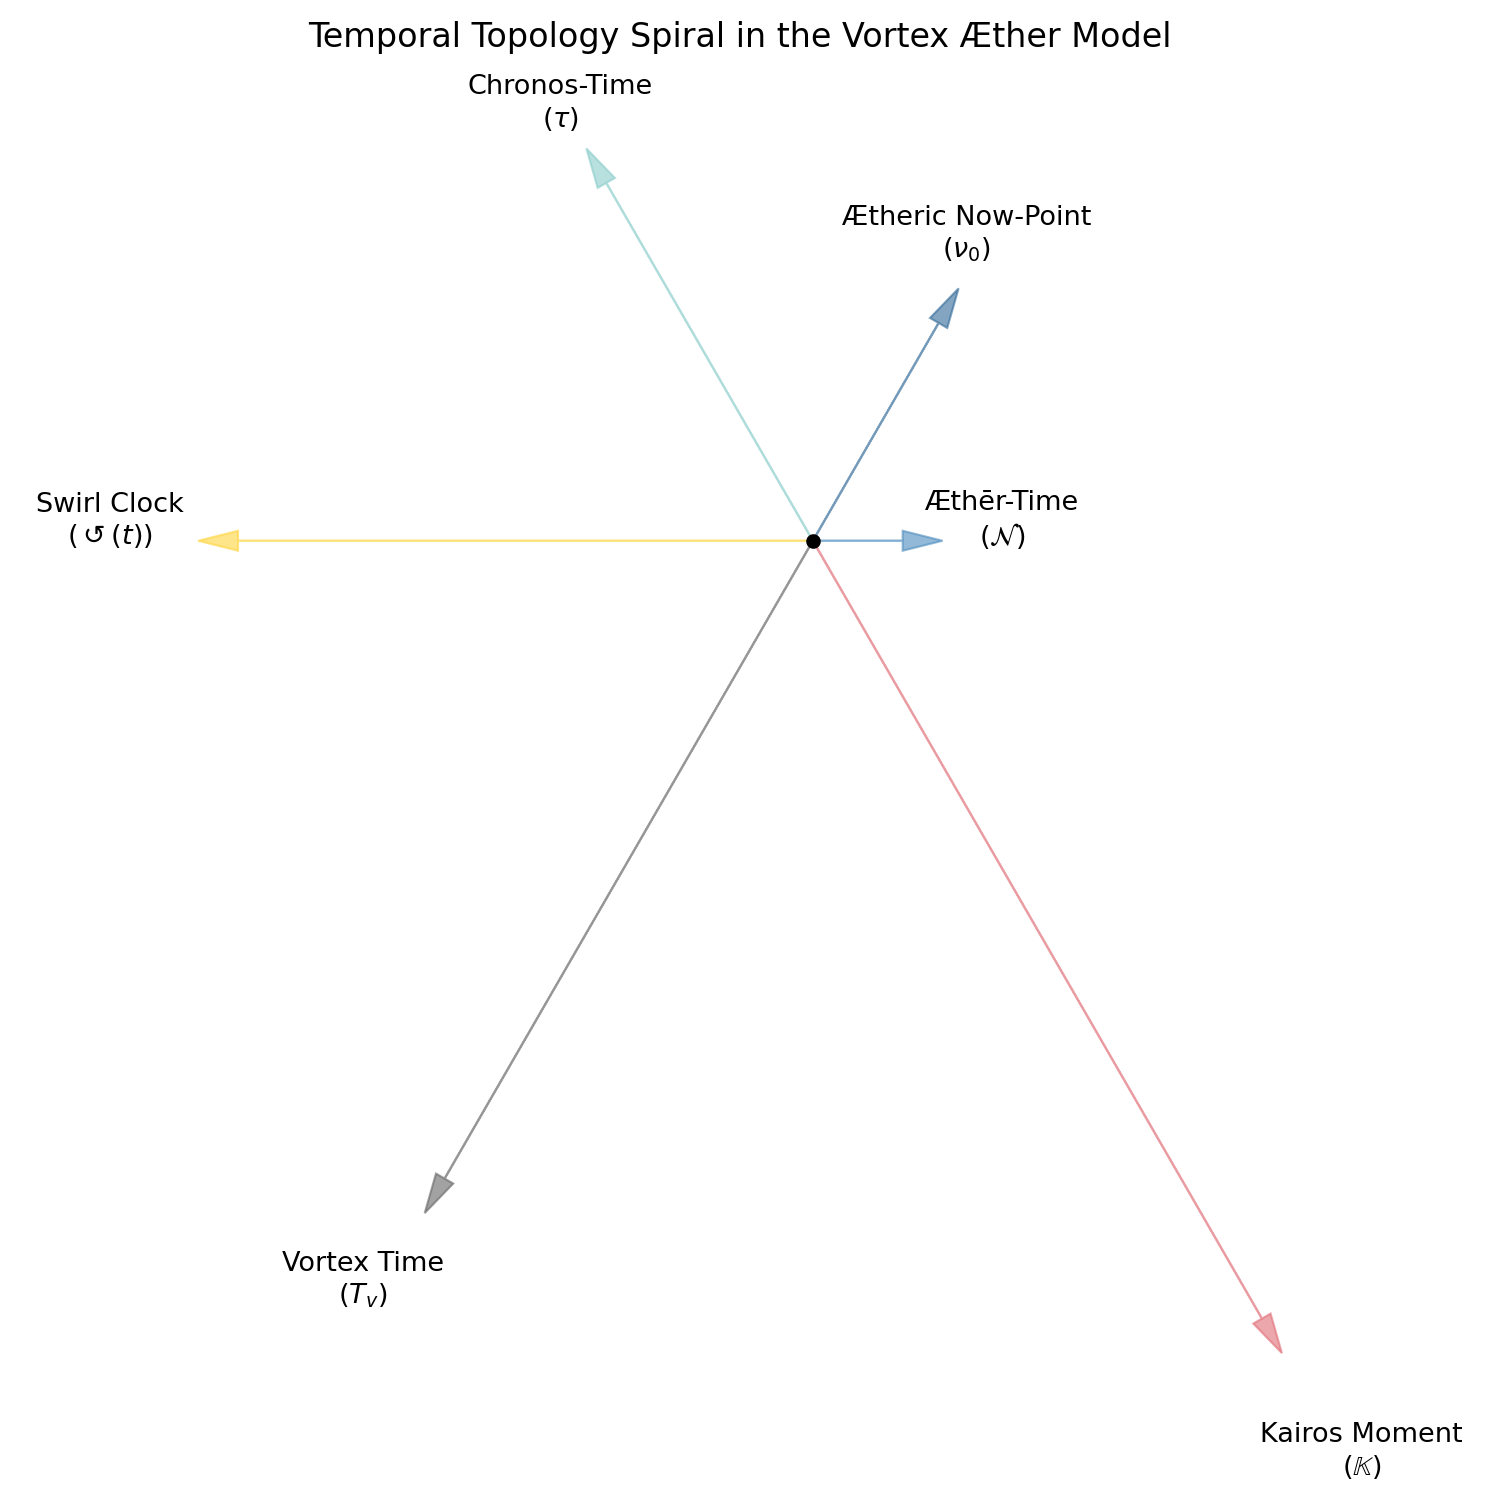
\includegraphics[width=0.65\textwidth]{images/TimeConstruct} % insert your generated swirl diagram here
    \caption{Temporal Topology in the Vortex Æther Model (VAM). All constructs of time emerge radially from a central ætheric origin. Each node represents a different mode of temporal existence in the VAM framework.}
    \label{fig:temporal_swirl}
\end{figure}

\subsection{Mathematical Definitions}

We define the following cornerstone temporal equations:

\begin{enumerate}
    \item \textbf{Chronos-Time evolution:}
    \begin{equation}
        \frac{d\tau}{d\mathcal{N}} = \gamma^{-1}(\vec{v})
    \label{eq:chronos_time}
    \end{equation}

    \item \textbf{Swirl Clock gradient dynamics:}
    \begin{equation}
        \nabla S(t) = \frac{\partial \vec{S}}{\partial \mathcal{N}} + \omega(\tau)\hat{n}
    \label{eq:swirl_clock}
    \end{equation}

    \item \textbf{Æther-relative field tensor modulation:}
    \begin{equation}
        F^{\mu\nu}(\Xi_0) = \partial^\mu A^\nu - \partial^\nu A^\mu + \phi(\circlearrowleft)\delta^{\mu\nu}
    \label{eq:Æther-field_tensor}
    \end{equation}

    \item \textbf{Ætheric causality surface:}
    \begin{equation}
        \Sigma_{\nu_0} = \{ x^\mu \mid \tau(x) = \mathcal{N} \}
    \label{eq:Æther-causality}
    \end{equation}

    \item \textbf{Energy conservation with Kairos trigger:}
    \begin{equation}
        \frac{dE}{d\mathcal{N}} + \nabla \cdot \vec{J} = \mathbb{K}(\vec{x}, \tau)
    \label{eq:Kairos_energy}
    \end{equation}
\end{enumerate}

These equations formalize how temporality in VAM emerges from vortex energetics, field topology, and critical transitions.

\subsection{Interpretation of Temporal Constructs}

Each temporal construct serves distinct roles:
\begin{itemize}
    \item \textbf{Æther-Time $(\mathcal{N})$:} Foundation for universal causality.
    \item \textbf{Chronos-Time $(\tau)$:} Measures local dilations in vortex fields.
    \item \textbf{Swirl Clock $(S(t))$:} Defines cyclic stability and identity of vortex particles.
    \item \textbf{Vortex Proper Time $(T_v)$:} Determines internal loop resonances and knot stability.
    \item \textbf{Kairos Moments $(\mathbb{K})$:} Marks measurable critical transitions such as quantum jumps and vortex reconnections.
\end{itemize}

\subsection{Practical and Experimental Relevance}

Temporal constructs enable precise experimental predictions:
\begin{itemize}
    \item \textbf{Chronos-Time} provides measurable dilations testable via atomic clocks in rotating superfluids.
    \item \textbf{Kairos Moments} predict discrete energy transitions observable in controlled vortex experiments, potentially providing empirical signatures differentiating VAM from classical models.
\end{itemize}

This structured temporal framework not only clarifies the theoretical underpinning of VAM but significantly enhances experimental testability.


\section{Temporal-Topological Dynamics in the Vortex Æther Model}

\subsection*{Equation (1): Ætheric Energy Conservation with Kairos Trigger}
\begin{equation}
    \frac{dE}{d\mathcal{N}} + \nabla \cdot \vec{J} = \mathbb{K}(\vec{x}, \tau)
    \label{eq:Kairos_trigger_energy_conservation}
\end{equation}

\textbf{Interpretation:} The rate of energy change in universal time $\mathcal{N}$ is balanced by flux divergence and a local ``Kairos event'' $\mathbb{K}$. When $\mathbb{K} \neq 0$, topological transitions (e.g., knot formation, decay) occur—this term models time-symmetric violations or energy "pinches."

\subsection*{Equation (2): Swirl Clock Phase Evolution}
\begin{equation}
    \nabla \vec{S}(t) = \frac{d}{d\mathcal{N}} \vec{S}(t) + \omega(\tau) \hat{n}
\label{eq:Swirl_clock_phase_evolution}
\end{equation}

\textbf{Interpretation:} The spatial gradient of the internal swirl phase $\vec{S}(t)$ is composed of a universal clock drift plus intrinsic vortex angular velocity. $\omega(\tau)$ is locally defined, modulated by proper time $\tau$.

\subsection*{Equation (3): Æther-Modulated Field Tensor}
\begin{equation}
    F^{\mu\nu} = \partial^\mu A^\nu - \partial^\nu A^\mu + \phi(\circlearrowleft) \delta^{\mu\nu}
\label{eq:Æther_modulated_field_tensor}
\end{equation}

\textbf{Interpretation:} This modified gauge field equation includes a scalar modulation based on internal swirl phase, representing helicity injection or topological memory from prior knot interactions.

\subsection*{Unified Interpretation}
Together, these equations constitute the dynamic triad of the Vortex Æther Model: energy, phase, and field interactions modulated through temporal flow ($\mathcal{N}, \tau$) and internal vortex topology.

\subsection*{Concrete Examples}

\subsubsection*{Example 1: Trefoil Vortex and Energy Dissipation}
Consider a trefoil knot vortex with $T_v = 1.5 \times 10^{-21}$ s, circulation $\Gamma = 6.6 \times 10^{-8} \text{ m}^2/\text{s}$, and flux divergence $\nabla \cdot \vec{J} = 1.2 \times 10^{-13} \text{ W/m}^3$. At a Kairos moment $\mathbb{K} = 3.3 \times 10^{-12} \text{ W/m}^3$, the net energy change is $2.1 \times 10^{-12} \text{ W/m}^3$, indicating topological energy restructuring.

\subsubsection*{Example 2: Swirl Clock Interference}
Two vortex clocks with frequencies $\omega_1 = 4\pi$ rad/s and $\omega_2 = 5\pi$ rad/s produce interference with a beat structure occurring at integer multiples of 2 s. This illustrates phase coherence phenomena relevant to quantum spinor analogies.

\subsubsection*{Example 3: Swirl-Modified Gauge Field}
With vector potential $A_x = e^{-x^2}\cos(\omega t)$ and swirl potential $\phi(\circlearrowleft) = \lambda\sin(\theta)$, the gauge field tensor component $F^{10}$ becomes swirl-phase-modulated, demonstrating how internal angular structures influence observable fields.

\section*{Visualizing Temporal Dynamics in VAM}

\subsection*{1. Swirl Clock Interference Pattern}
\begin{figure}[H]
    \centering
    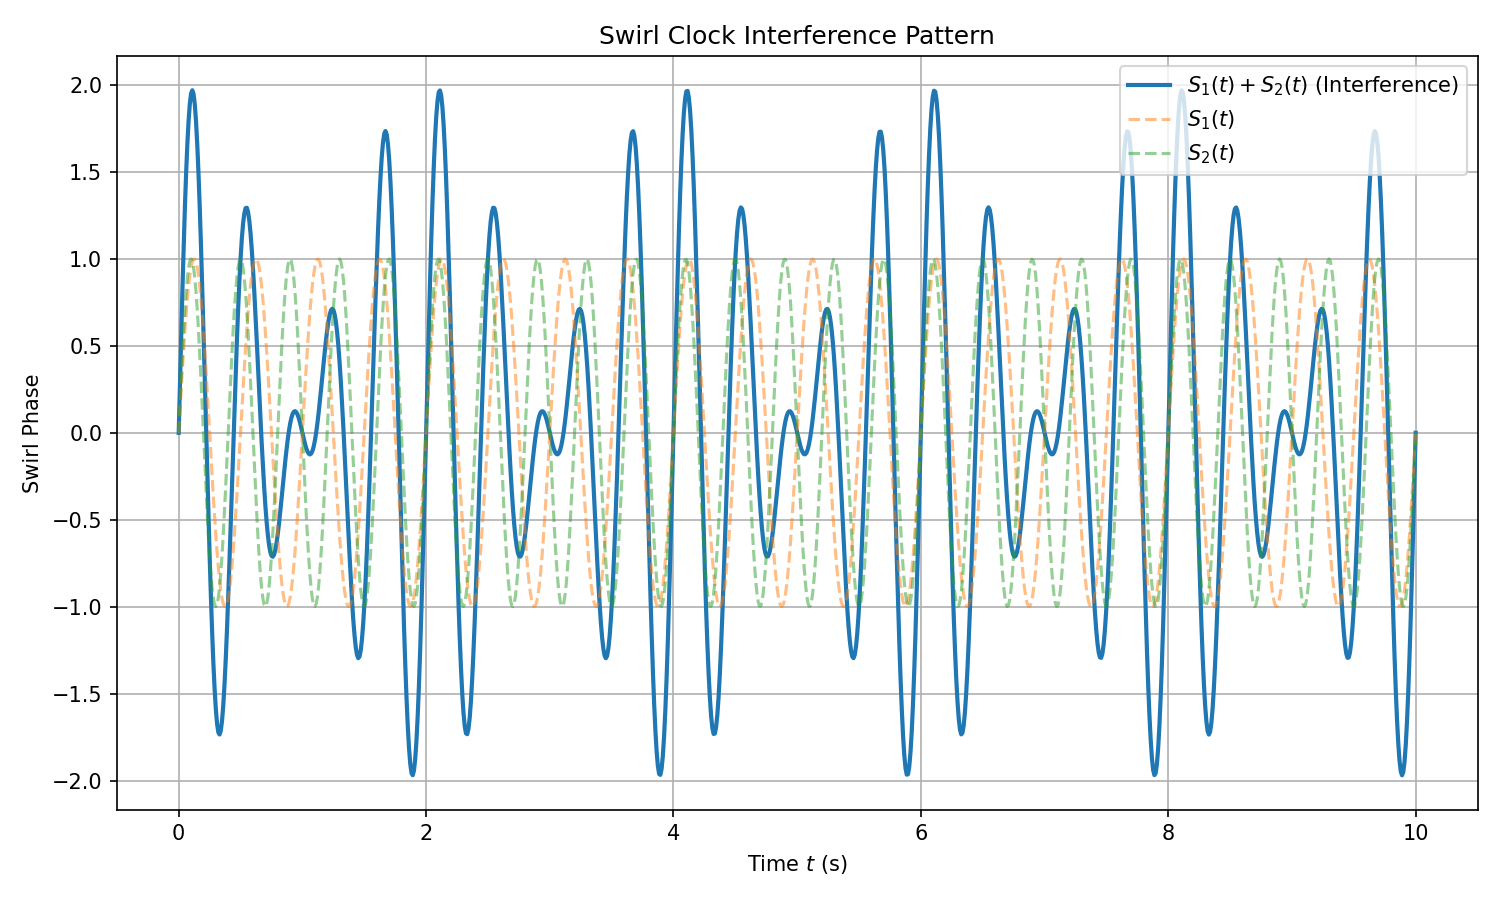
\includegraphics[width=0.8\textwidth]{images/SwirlClockInterference}
    \caption{Interference between two swirl clocks with angular frequencies $\omega_1 = 4\pi$ and $\omega_2 = 5\pi$. The phase difference leads to beat structures and modulation patterns—analogous to quantum spinor dynamics and timing gates in ætheric systems.}
    \label{fig:swirl_interference}
\end{figure}

\subsection*{2. Energy Growth from Kairos Moment}
\begin{figure}[H]
    \centering
    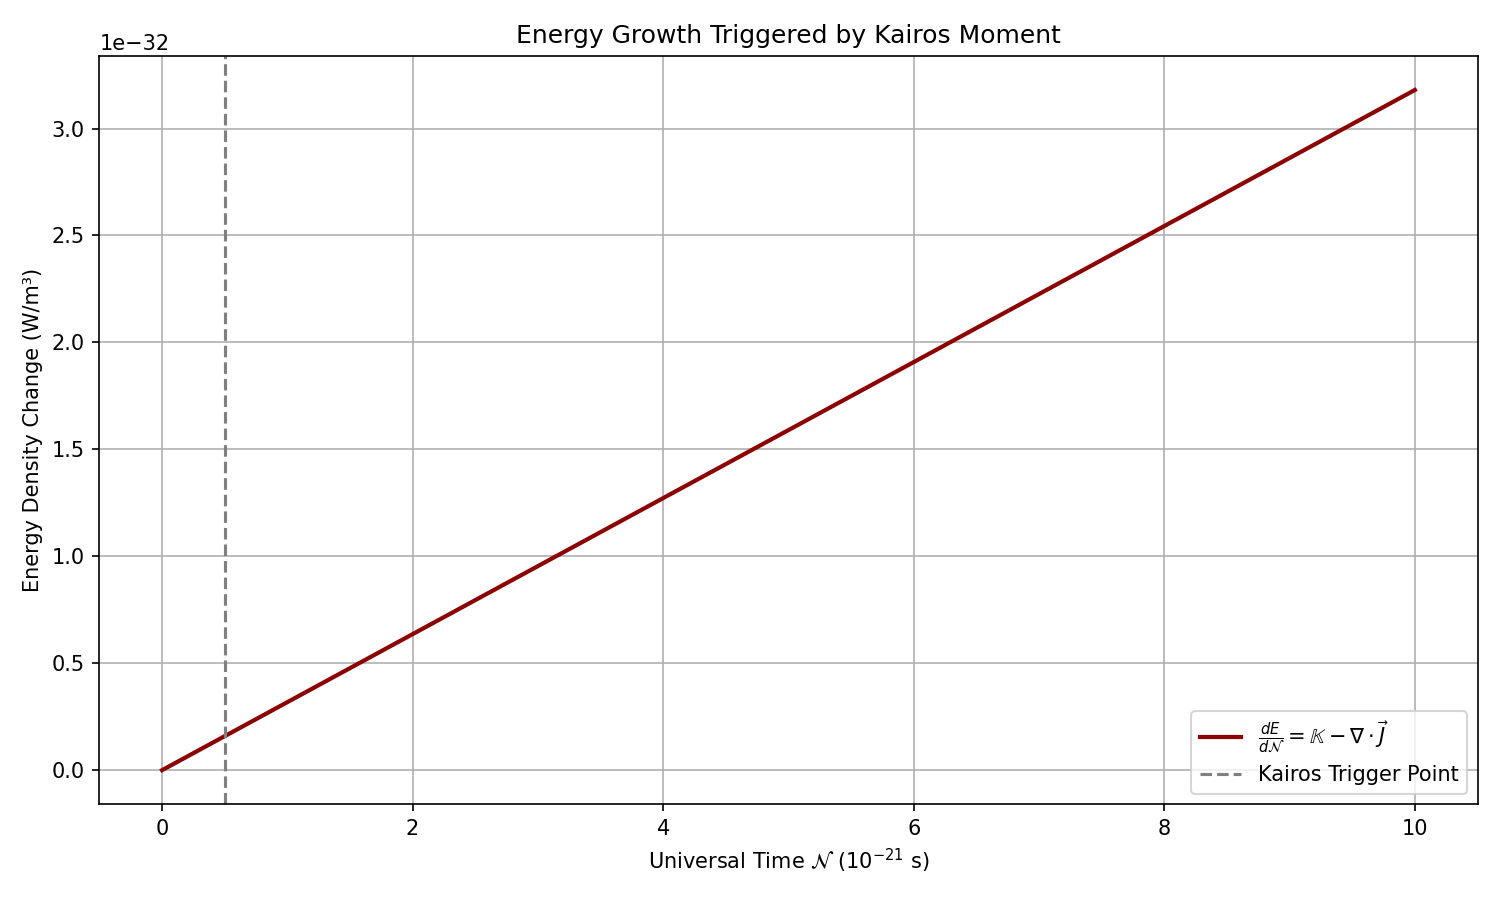
\includegraphics[width=0.8\textwidth]{images/SwirlClockInterference2}
    \caption{Temporal evolution of energy density in æther, showing energy injection at a Kairos moment ($\mathbb{K}$) minus the divergence of energy flux $\nabla \cdot \vec{J}$. The slope reflects the conservation law $\dv{E}{\mathcal{N}} + \nabla \cdot \vec{J} = \mathbb{K}$.}
    \label{fig:kairos_energy}
\end{figure}

\subsection*{3. Swirl-Modulated Field Tensor}
\begin{figure}[H]
    \centering
    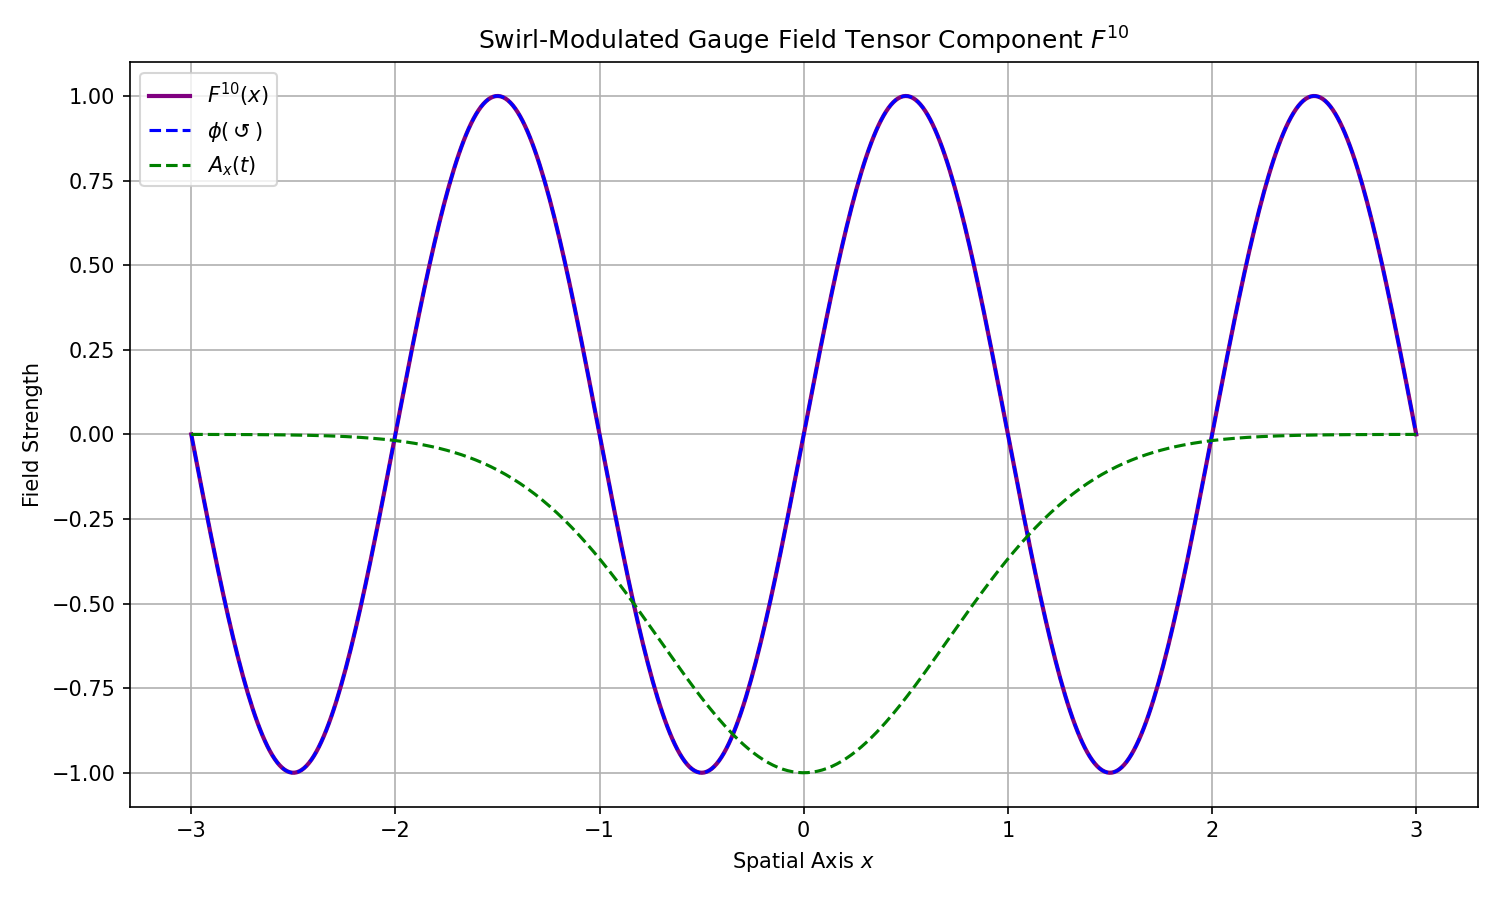
\includegraphics[width=0.8\textwidth]{images/SwirlClockInterference3}
    \caption{Spatial variation of the gauge field tensor component $F^{1 0}$ under the influence of a swirl-phase-modulated potential $\phi(\circlearrowleft) = \lambda \sin(\theta(x))$ and a vector potential $A_x(t) = e^{-x^2} \cos(\omega t)$. This illustrates how topological internal structures alter observable field properties.}
    \label{fig:swirl_tensor}
\end{figure}
